% ============================================================================
%  Dynamics of the Five-Organ Diagram in Chinese Medicine
%  Full draft. Compile with XeLaTeX (ctex requires it).
%
%  NOTE: The network-motif analysis is deliberately left as a stub
%        (Section \ref{sec:motifs}) for the author to write.
% ============================================================================
\documentclass[11pt]{article}

\usepackage{amsmath}
\usepackage{amsfonts}
\usepackage{amssymb}
\usepackage{amsthm}
\usepackage{graphicx}
\usepackage{booktabs}
\usepackage{ctex}          % Chinese characters; requires XeLaTeX
\usepackage[usenames,dvipsnames]{xcolor}
\usepackage{tikz}
\usetikzlibrary{arrows,backgrounds}
\usepackage{hyperref}
\usepackage{caption}

\hypersetup{colorlinks=true,linkcolor=blue!55!black,citecolor=blue!55!black,
            urlcolor=blue!55!black}

\pagestyle{plain}
\textheight235truemm\textwidth165truemm
\voffset-2.2cm\hoffset-1.2cm \vfuzz=10000truept\hfuzz=10000truept

\newcommand{\RED}[1]{{\color{red}{#1}}}
\newcommand{\ignore}[1]{}
\newcommand{\R}{{\mathbb{R}}}
\newcommand{\Z}{{\mathbb{Z}}}

\newtheorem{theorem}{Theorem}[section]
\newtheorem{lemma}[theorem]{Lemma}
\newtheorem{definition}[theorem]{Definition}
\newtheorem{corollary}[theorem]{Corollary}
\newtheorem{proposition}[theorem]{Proposition}
\newtheorem{remark}[theorem]{Remark}
\newtheorem{example}[theorem]{Example}

\tikzstyle{place}=[circle,draw=blue!50,fill=blue!20,thick]

\usepackage[backend=biber,style=alphabetic,sorting=ynt]{biblatex}
\addbibresource{Chinese_med.bib}

\title{Dynamics of the Five-Organ Diagram in Chinese Medicine:\\
Saturating Interactions and the Stability of the Balanced State}
\author{Carter Feng and Yunjiao Wang}

\begin{document}
\maketitle

\begin{abstract}
The five-element (Wu-Xing) system is the theoretical backbone of Traditional
Chinese Medicine (TCM), and several continuous-time models of it have been
proposed. Almost all adopt Lotka--Volterra (bilinear, mass-action) couplings.
We show that this choice has a decisive consequence: in the bilinear setting the
\emph{balanced} state, in which all five organs carry equal activity, is
generically unstable, so the model has no dynamical representation of sustained
health. We first reproduce the bilinear analysis of Lin and Han~\cite{Lin2020}
exactly, and in doing so identify three errors in their reported stability
computations: a periodic solution reported as unstable is in fact an
asymptotically stable limit cycle; a fixed point reported as unstable is
neutrally stable with two exactly-zero eigenvalues; and a case reported as
chaotic is quasiperiodic on a three-dimensional invariant surface, for which we
derive two conserved quantities. We then propose a model in which the Sheng
(generating) and Ke (over-acting) interactions saturate, each term being
justified by a named TCM relation. For this model we prove that a unique
positive balanced state exists whenever $a+c>g$, that all trajectories remain in
an attracting invariant box (so no parameter tuning is needed to avoid
non-physiological blow-up), and that the Jacobian at the balanced state is
circulant, which yields its eigenvalues in closed form through the discrete
Fourier transform and separates uniform from symmetry-breaking perturbations. At
baseline parameters the balanced state is asymptotically stable. Across
randomised parameter studies under three sampling priors---including one
constructed to be maximally favourable to the bilinear model---the saturating
model has a stable balanced state in over 90\% of draws against at most 47\% for
the bilinear model. We report the limitations of each test explicitly, including
an ablation showing that the extra term carried by the bilinear model helps
rather than handicaps it.
\end{abstract}

\tableofcontents
\newpage

% ============================================================================
\section{Introduction}
% ============================================================================

Traditional Chinese medicine (TCM) has been widely recognized and has become an
invaluable component of alternative medicine in the West~\cite{Kaptchuk2000},
though it is not always viewed correctly. Chinese medicine is the result of
science over a long period, being the product of continuous critical thinking
and extensive clinical observation and testing~\cite{Kaptchuk2000}. It is a
coherent and independent system of thought and practice developed over two
thousand years. As Manfred Porkert~\cite{Porkert1990} rightly pointed out,
Chinese medicine is not less logical than Western medicine, merely less
analytical. In this project we aim to contribute an analytical study of Chinese
medicine.

The distinguishing feature of TCM is that it is \emph{holistic}: the body is
modelled not as a collection of independent organs but as a network of
interacting subsystems, so that a disorder in one organ is expected to
propagate to others along specific, named channels. This is the content of the
five-element or Wu-Xing diagram, which specifies two directed cycles on five
nodes---one of generation (Sheng, 生) and one of control (Ke, 克). Diagnostic
and therapeutic principles are stated directly in terms of these channels, for
example 虚则补其母 (``if the child is deficient, tonify the mother'').

A natural question is whether these principles can be given a quantitative
dynamical formulation. Several authors have attempted this, and we survey their
work in Section~\ref{sec:lit}. The overwhelmingly dominant modelling choice is
to represent every inter-organ interaction by a \emph{bilinear} (mass-action)
product $x_ix_j$, in direct analogy with Lotka--Volterra population dynamics.
This is a reasonable first step, and it has produced a rich catalogue of
behaviours: fixed points, limit cycles, and chaos.

It has also produced a persistent and, we argue, fatal difficulty. In the
bilinear setting the balanced state---the state in which all five organs carry
the same level of activity, and the obvious candidate for a mathematical image
of health---is typically \emph{unstable}. Lin and Han~\cite{Lin2020} state this
outright, reporting that every case they examined was unstable. A model in which
the balanced state is unstable cannot represent a body that is well and stays
well: perturb it and the organs diverge from one another permanently. Since
maintaining health, rather than describing collapse, is the central concern of
TCM, this is a serious mismatch between the mathematics and its subject.

\subsection{Contributions}

This paper makes the following contributions.

\begin{enumerate}
\item \textbf{Exact reproduction of the bilinear analysis.} We reimplement the
symmetric model of Lin and Han~\cite{Lin2020} and recover their equilibria,
their Jacobian eigenvalues to every published decimal, and their reported period
$T\approx 17.626$.

\item \textbf{Three corrections.} Using the variational (tangent-space) method
with $QR$ reorthonormalization in place of a singular-value estimate applied to a
time series, we show that (i) their ``unstable'' periodic solution is an
asymptotically stable limit cycle, (ii) their ``unstable'' fixed point is
neutrally stable with two exactly-zero eigenvalues, and (iii) their ``chaotic''
case is quasiperiodic, being confined by two conserved quantities that we derive
in closed form and verify to machine precision.

\item \textbf{A saturating model with term-by-term justification.} We replace
the bilinear Sheng and Ke over-acting terms with saturating ones, and justify
each modification by a specific classical relation rather than by mathematical
convenience.

\item \textbf{Analytic results.} We prove existence and uniqueness of a positive
balanced state under the mild condition $a+c>g$; we exhibit an attracting
invariant box, so that positivity and boundedness hold for \emph{all} parameter
values; and we show that the Jacobian at the balanced state is circulant,
giving its eigenvalues in closed form and separating uniform from
symmetry-breaking modes.

\item \textbf{Randomised comparison with a justified prior.} We compare the two
models over thousands of random parameter draws under three sampling priors,
including a physiologically ordered one. We show that the ordering
\emph{improves} the bilinear model's performance, so that the comparison is
conservative, and that the conclusion is nonetheless unchanged.

\item \textbf{Explicit limitations.} We report where each test is weak, including
an ablation demonstrating that the additional term carried by the bilinear model
is an advantage rather than a handicap, and a quantification of how strongly the
long-run classification depends on initial conditions.
\end{enumerate}

The network-motif analysis, which interprets the classical treatment principles
as statements about two- and three-node subnetworks, is developed separately in
Section~\ref{sec:motifs}.

% ============================================================================
\section{Literature Review}\label{sec:lit}
% ============================================================================

The five-element system has been modelled by both discrete and continuous
dynamical systems.

\paragraph{Discrete models.}
In~\cite{Bellavite1998} the five-element network is modelled by a synchronous
Boolean network in which each node receives two inputs, one activating
(generating/Sheng) and one inhibiting (restraining/Ke). A node is either active
(ON) or inactive (OFF) at the next time step according to the state of its two
inputs; when both inputs agree, the node is set ON or OFF by an arbitrary
convention that characterises the system. That paper also studies the system
with delays and perturbations. However, it does not connect the results back to
the physiological system: it is not clear whether the patterns exhibited make
sense or carry meaning. The system has also been modelled by discrete dynamical
systems in which each node takes three states---normal, excess, and
deficiency~\cite{Lin2020}.

\paragraph{Continuous models.}
A recent paper by Nian et al.~\cite{Nian2025} proposes a system of the form
\[
\begin{array}{rl}
\frac{dM}{dt} &= a_1 M + b_1 S+ c_1 J + d_1 HTSJ \\
\frac{dH}{dt} &= a_2 H + b_2 M+ c_2S   + d_2 MTSJ \\
\frac{dT}{dt} &= a_3 T + b_3 H+ c_3 M + d_3 HMSJ \\
\frac{dJ}{dt} &= a_4 J + b_4 T + c_4 H + d_4 HTSM \\
\frac{dS}{dt} &= a_5 S + b_5 J+ c_5 T + d_5 HTMJ .
\end{array}
\]
All of the coefficients $a_i$, $b_i$ and $c_i$ are set to unity, which removes
any distinction between the strengths of physiologically quite different
relations and is difficult to justify.

The most systematic continuous treatment is that of Lin and
Han~\cite{Lin2020}, which we take as our point of comparison throughout. They
enumerate six influences acting on each element---``gain'', ``saturation'',
``generating'', ``is-generated'', ``restricting'' and ``is-restricted''---and
build a symmetric five-dimensional system containing all six. They report that,
across 300 randomly generated configurations, the system converges to a fixed
point or a periodic solution, or becomes chaotic. They analyse stability using
the first Lyapunov method and Lyapunov exponents, and dissipativity via the rate
of change of phase-space volume.

\paragraph{What the literature does not do.}
Two gaps motivate the present work. First, almost every continuous model uses
bilinear couplings, and we show in Section~\ref{sec:stability} that this choice
alone is enough to destabilise the balanced state. Second, few of these papers
check whether their models reproduce the \emph{named} pathological relations of
the classics---相乘 (over-acting), 相侮 (rebellious counter-acting), 母病及子
(mother-illness reaching the child), 子盗母气 (the child stealing the mother's
qi). Producing dynamics is not the same as producing TCM.

% ============================================================================
\section{Relations in Wu-Xing and Mathematical Modelling}\label{sec:relations}
% ============================================================================

\subsection{The Five Organs and Index Assignment}

We index the five organs as follows, following the standard Wu-Xing cycle:

\begin{center}
\begin{tabular}{cll}
\toprule
Index & Element & Organ \\
\midrule
$x_1$ & Wood\; (木) & Liver\; (肝) \\
$x_2$ & Fire\; (火)  & Heart\; (心) \\
$x_3$ & Earth\; (土) & Spleen\; (脾) \\
$x_4$ & Metal\; (金) & Lung\; (肺) \\
$x_5$ & Water\; (水) & Kidney\; (肾) \\
\bottomrule
\end{tabular}
\end{center}

Let $x_i = x_i(t) \geq 0$ denote the functional activity level (qi) of organ $i$
at time $t$. All indices are understood modulo $5$.

\subsection{Fundamental Relationships}

TCM identifies three primary inter-organ relationships, each of which
contributes a term to the dynamical model.

\medskip
\noindent\textbf{Sheng (生, Generating) cycle.}
Each organ nourishes the next in the cycle
\[
x_1 \to x_2 \to x_3 \to x_4 \to x_5 \to x_1 .
\]
Each organ is the \textbf{mother} of the next organ in the cycle, and the next
is the \textbf{child}. We denote the \emph{Sheng mother} of organ $i$ by
$\sigma(i)$:
\[
\sigma(1)=5,\quad \sigma(2)=1,\quad \sigma(3)=2,\quad \sigma(4)=3,\quad \sigma(5)=4 .
\]

\medskip
\noindent\textbf{Ke (克, Controlling) cycle.}
Each organ restrains another following the pentagram pattern
\[
x_1 \to x_3 \to x_5 \to x_2 \to x_4 \to x_1 .
\]
We denote the \emph{Ke target} of organ $i$ (the organ that $i$ controls) by
$\kappa(i)$, and the \emph{Ke controller} of organ $i$ (the organ that controls
$i$) by $\rho(i)$:

\begin{center}
\begin{tabular}{cll}
\toprule
Organ $i$ & Ke target $\kappa(i)$ & Ke controller $\rho(i)$ \\
\midrule
$x_1$ Wood  & $x_3$ Earth  & $x_4$ Metal  \\
$x_2$ Fire  & $x_4$ Metal  & $x_5$ Water  \\
$x_3$ Earth & $x_5$ Water  & $x_1$ Wood   \\
$x_4$ Metal & $x_1$ Wood   & $x_2$ Fire   \\
$x_5$ Water & $x_2$ Fire   & $x_3$ Earth  \\
\bottomrule
\end{tabular}
\end{center}

Equivalently, in the cyclic labelling,
\begin{equation}\label{eq:maps}
\sigma(i)=i-1,\qquad \sigma^{-1}(i)=i+1,\qquad \rho(i)=i-2,\qquad \kappa(i)=i+2 .
\end{equation}
Equation~\eqref{eq:maps} is used throughout and is the single fact needed to read
every subsequent formula.

\begin{figure}[!htb]
\centering
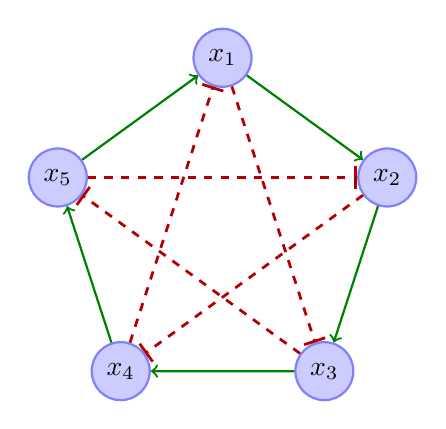
\begin{tikzpicture}[line width=1pt, scale=2.2]
\node[place] (M) at (90:1) {$x_1$};
\node[place] (H) at (18:1) {$x_2$};
\node[place] (T) at (-54:1) {$x_3$};
\node[place] (J) at (234:1) {$x_4$};
\node[place] (S) at (162:1) {$x_5$};
\path[->,green!50!black,thick]
      (M) edge (H) (H) edge (T) (T) edge (J) (J) edge (S) (S) edge (M);
\path[-|,red!70!black,dashed]
      (M) edge (T) (T) edge (S) (S) edge (H) (H) edge (J) (J) edge (M);
\end{tikzpicture}
\caption{The Wu-Xing network. Solid green arrows are the Sheng (generating)
cycle around the outer pentagon; dashed red bars are the Ke (controlling) cycle
forming the inner pentagram. Every organ has exactly one mother, one child, one
controller and one target.}
\label{fig:network}
\end{figure}

\medskip
\noindent\textbf{Wu (侮, Rebellious Counter-Acting).}
Under pathological conditions, when organ $i$ becomes severely deficient, or when
the organ it normally controls, $x_{\kappa(i)}$, is over-active, the controlled
organ may rebel against $x_i$, exerting a reverse draining effect once $x_i$
falls below a threshold governed by $\epsilon_i>0$. A convenient form is
\[
-\,\frac{b_i\,x_{\kappa(i)}}{1+\epsilon_i x_i}.
\]
The classics grade the two abnormal Ke relations explicitly: over-acting (相乘)
is 贼邪, the ``thief evil'', which \emph{greatly} weakens its object, whereas
rebellion (相侮) is 微邪, the ``mild evil'', which only \emph{mildly} weakens it.
We record this grading here because it constrains the relative sizes of the
corresponding coefficients (Section~\ref{sec:ordering}). The analysis in this
paper concerns the model without the Wu term; incorporating it is discussed in
Section~\ref{sec:future}.

\subsection{The complete list of relations to be captured}

\paragraph{Sheng (generating).}
\begin{enumerate}
\item The mother nourishes the child, and the child draws back on the mother.
\item Deficiency in the mother leads to deficiency in the child (母病及子).
\item Excess in the mother leads to excess in the child.
\item Excess activity in the child leads to overdraw from the mother: the child
      consumes its element quickly and the mother must replenish more
      (子盗母气).
\item Weakness in the child eventually weakens the mother, because the child
      exhausts it over time.
\end{enumerate}

\paragraph{Ke (controlling).}
\begin{enumerate}\setcounter{enumi}{5}
\item Normal restraint: the controller suppresses its target. Under normal
      conditions this restraint is required to keep the target from growing
      without bound.
\item Over-acting (相乘, 贼邪): if the controller is in excess, or the target is
      deficient, the target is greatly weakened.
\item Rebellious counter-acting (相侮, 微邪): conversely, if the target is in
      excess or the controller deficient, the controller is mildly weakened.
\end{enumerate}

Relation~1 is the one that dictates the functional form of the Sheng term, and
it is where the bilinear and saturating models part company. The requirement
that a \emph{weak} child draws \emph{harder} on its mother means that the
nourishment rate must \emph{increase} as $x_i$ decreases. A bilinear term
$c\,x_i x_{\sigma(i)}$ does the opposite: it vanishes as the child is depleted.
A saturating term $c\,x_{\sigma(i)}/(1+x_i)$ has the required behaviour.
% ============================================================================
\section{The Bilinear Model and Its Reproduction}\label{sec:bilinear}
% ============================================================================

\subsection{The model of Lin and Han}

Lin and Han~\cite{Lin2020} assign each organ six influences, listed in
Table~\ref{tab:six}.

\begin{table}[!htb]
\centering
\begin{tabular}{clll}
\toprule
Symbol & Name & Meaning & Sign \\
\midrule
$a$ & gain        & self-production                      & $+$ \\
$b$ & saturation  & self-limitation                      & $-$ \\
$c$ & isG         & is generated by its mother           & $+$ \\
$d$ & isR         & is restricted by its controller      & $-$ \\
$g$ & G           & cost of generating its child         & $-$ \\
$h$ & R           & cost of restricting its target       & $-$ \\
\bottomrule
\end{tabular}
\caption{The six influences of the bilinear model.}
\label{tab:six}
\end{table}

In the symmetric case, in which all organs share parameter values, the model is
\begin{equation}\label{eq:lin}
\dot x_i \;=\; a x_i - b x_i^2
\;+\; c\,x_i x_{i-1}
\;-\; d\,x_i x_{i-2}
\;-\; g\,x_i x_{i+1}
\;-\; h\,x_i x_{i+2},
\qquad i\in\Z_5 .
\end{equation}

The structural point to note is that \emph{every} coupling in~\eqref{eq:lin} is a
product $x_ix_j$. This is mass-action, or Lotka--Volterra, form. No interaction
saturates: if the mother doubles, the nourishment delivered to the child
doubles, without limit.

\subsection{The balanced state}

Setting $x_i=x$ for all $i$ in~\eqref{eq:lin} collapses the system to the scalar
equation
\[
\dot x = a x + (c-b-d-g-h)x^2 = x\bigl(a + (c-b-d-g-h)x\bigr),
\]
so that, besides the origin, there is a unique balanced equilibrium
\begin{equation}\label{eq:linstar}
x^\ast=\frac{a}{M},\qquad M:=b+d+g+h-c .
\end{equation}
At $a=b=c=d=g=h=1$ this gives $x^\ast=1/3$.

\begin{remark}[Conditional boundedness]\label{rem:blowup}
Equation~\eqref{eq:linstar} requires $M>0$. The condition is not merely
technical. On the symmetric subspace, $\dot x = ax - Mx^2$; if $M<0$ the
quadratic term is \emph{positive} and $\dot x\approx |M|x^2$, which diverges in
finite time. Numerically, with $b=d=g=h=1$: $c=5$ (so $M=-1$) diverges at
$t\approx0.69$, and $c=4.1$ (so $M=-0.1$) at $t\approx2.35$; the same occurs
from asymmetric initial data. Thus the region in which the bilinear model
possesses a balanced state is exactly the region in which it is bounded. All
parameters examined in~\cite{Lin2020} satisfy $M>0$, so this behaviour does not
appear there, but it lies immediately outside the explored range.
\end{remark}

\subsection{Reproduction}

We reimplemented~\eqref{eq:lin} and its analytic Jacobian, and verified the
latter against finite differences at 200 random points (worst discrepancy
$2.4\times10^{-7}$, consistent with truncation error). We also verified the
equilibrium formula by substitution, obtaining $|F(x^\ast)|\le 9\times10^{-13}$.

\paragraph{Case 1: eigenvalues at the balanced state.}
Linearising at $x^\ast=1/3$ with all parameters equal to unity gives the
eigenvalues in Table~\ref{tab:case1}. The agreement with~\cite{Lin2020} is exact
to every published decimal, confirming that our equations and index maps
coincide with theirs.

\begin{table}[!htb]
\centering
\begin{tabular}{ll}
\toprule
Our computation & Reported in~\cite{Lin2020} \\
\midrule
$-1.0000$            & $-1$ \\
$-0.5393\pm 0.3919i$ & $-0.539\pm0.392i$ \\
$+0.2060\pm 0.6340i$ & $+0.206\pm0.634i$ \\
\bottomrule
\end{tabular}
\caption{Jacobian eigenvalues at the balanced state of the bilinear model,
$a=b=c=d=g=h=1$. Two eigenvalues have positive real part, so the balanced state
is unstable.}
\label{tab:case1}
\end{table}

\paragraph{Restriction only.}
Setting $d=h=1$ and $a=b=c=g=0$ removes all generation. Every term is then
negative and activity can only decay. Starting from $(1,2,3,4,5)$ the solution
decays monotonically to $(0,\,0,\,0.0003,\,2.3426,\,1.3041)$: three organs reach
zero, as reported. The surviving pair is precisely the pair with no restraining
link between them.

\paragraph{The periodic case.}
With all parameters equal to unity and the same initial data, the system settles
onto a cycle in which the five organs pulse in a staggered wave, each peaking one
fifth of a period after its Sheng mother. Measuring the period from the spacing
of peaks of $x_2$ after discarding the transient gives $T=17.626$, matching the
reported value.

\paragraph{The irregular case.}
With $c=g=1$ and the remaining parameters zero, the trajectory becomes
irregular and the phase portraits of $x_2$ against the other coordinates fill
rounded triangular regions, reproducing the published figures.

% ============================================================================
\section{Three Corrections to the Published Stability Analysis}\label{sec:corrections}
% ============================================================================

Having reproduced every published number that we could check, we turned to the
stability computations. Three do not survive scrutiny. We record the corrections
because they bear directly on the question of whether a balanced state can be
stable.

\subsection{A structural constraint on Lyapunov spectra}

For a smooth autonomous system $\dot x = F(x)$, any bounded trajectory that is
not an equilibrium possesses at least one Lyapunov exponent exactly equal to
zero, corresponding to the direction along the flow: a perturbation that merely
advances a point along its own orbit neither grows nor decays. Consequently
every spectrum reported for a limit cycle, a torus, or a chaotic attractor
\emph{must} contain a zero. The two spectra reported in~\cite{Lin2020},
\[
\{0.3885,\,-0.1719,\,-0.3473,\,-0.6833,\,-0.9731\}
\quad\text{and}\quad
\{0.6700,\,0.6606,\,-0.0761,\,-0.0794,\,-1.1751\},
\]
contain no zero exponent and therefore cannot be correct as stated.

\subsection{Method}

We compute Lyapunov spectra by the variational (tangent-space) method: the five
state equations are integrated together with five tangent vectors evolving under
the Jacobian, and the tangent frame is periodically reorthonormalised by a $QR$
decomposition, the logarithms of the diagonal stretch factors being accumulated.
Two details carry the weight. First, an initial transient is discarded so that
the asymptotic rate is measured rather than the approach to the attractor.
Second, the $QR$ step is essential: without it every tangent vector collapses
onto the fastest-growing direction and one recovers $\lambda_{\max}$ five times
instead of five distinct exponents.

\subsection{Correction 1: the periodic solution is stable}

Recomputing at $a=b=c=d=g=h=1$ gives
\[
\{0.0011,\,-0.1232,\,-0.2721,\,-0.2728,\,-0.9998\},
\]
exactly one zero exponent and four negative ones. This is the signature of an
\emph{asymptotically stable} limit cycle, not of the unstable periodic solution
reported. The period agrees with~\cite{Lin2020}. We attribute the discrepancy to
a singular-value estimate applied over a window that included the transient
from $(1,2,3,4,5)$.

\subsection{Correction 2: the fixed point is neutrally stable}

For the restriction-only case the reported exponents
$\{0.0015,\,0.0006,\,-1.3159,\,-2.3517,\,-3.7092\}$ were read as containing two
positive values. Evaluating the Jacobian at the attained final state
$(0,0,0,2.3426,1.3038)$ gives instead
\[
\{0,\;0,\;-1.3038,\;-2.3426,\;-3.6464\},
\]
where the two zeros are structurally exact: coordinates resting at $x_i=0$
generate genuinely degenerate directions. The three negative eigenvalues agree
with the reported values to within roughly one percent, which identifies the
reported ``positive'' entries as numerical noise at the $10^{-3}$ level. The
correct conclusion is neutral stability. This is consistent with the trajectory
converging; as published, the case is described simultaneously as convergent and
unstable, which cannot both hold.

\subsection{Correction 3: the chaotic case is quasiperiodic}

Setting $c=g=1$ with $a=b=d=h=0$ reduces~\eqref{eq:lin} to
\begin{equation}\label{eq:conserv}
\dot x_i = x_i\bigl(x_{i-1}-x_{i+1}\bigr), \qquad i\in\Z_5 .
\end{equation}

\begin{proposition}\label{prop:conserved}
System~\eqref{eq:conserv} admits the two independent conserved quantities
\[
I_1=\sum_{i} x_i, \qquad I_2=\prod_{i} x_i .
\]
\end{proposition}

\begin{proof}
Summing~\eqref{eq:conserv} over $i$, the right-hand side telescopes around the
cycle, giving $\frac{d}{dt}\sum_i x_i=0$. For the product, on the positive
orthant,
\[
\frac{d}{dt}\log\prod_i x_i=\sum_i\frac{\dot x_i}{x_i}
=\sum_i\bigl(x_{i-1}-x_{i+1}\bigr)=0 . \qedhere
\]
\end{proof}

We verified both invariants numerically, with relative drift of order
$10^{-15}$. Two conserved quantities confine the motion to a three-dimensional
invariant surface within the five-dimensional state space; in particular no
attractor exists, since the flow is volume-preserving.

Moreover the largest exponent computed over increasing horizons decays as
$1/T$:
\[
\lambda_{\max}(T{=}500)=0.0120,\qquad
\lambda_{\max}(T{=}1000)=0.0070,\qquad
\lambda_{\max}(T{=}2000)=0.0038,
\]
halving as $T$ doubles, which is the signature of an exponent converging to zero
rather than to the reported $0.67$. The dynamics are therefore quasiperiodic on
a torus, not chaotic.

\subsection{Consequence}

These corrections strengthen rather than weaken the motivation for the present
work. Even after correction, the bilinear model has no asymptotically stable
\emph{balanced} state: at $a=b=c=d=g=h=1$ the symmetric equilibrium retains
eigenvalues $0.206\pm0.634i$ with positive real part. Its attracting sets are
limit cycles or boundary states in which several organs vanish. Neither is a
satisfactory representation of sustained health.
% ============================================================================
\section{The Saturating Model}\label{sec:model}
% ============================================================================

\subsection{Formulation}

We propose the model
\begin{equation}\label{eq:sat}
\dot{x}_i \;=\;
\underbrace{a x_i - k x_i^2}_{\text{logistic self-regulation}}
\;+\;\underbrace{\frac{c\,x_{\sigma(i)}}{1+x_i}}_{\text{Sheng nourishment}}
\;-\;\underbrace{\frac{g\,x_i}{1+x_{\kappa(i)}}}_{\text{Ke over-acting}}
\;-\;\underbrace{h\,x_i x_{\rho(i)}}_{\text{Ke restraint}},
\qquad i\in\Z_5 .
\end{equation}

\subsection{Justification of each term}

\paragraph{Self-regulation, $a x_i - k x_i^2$.}
The linear term represents self-production proportional to current activity: a
more active organ regenerates faster. The quadratic term is crowding, giving a
finite carrying capacity. This is the standard one-node motif and is retained
unchanged from the bilinear model, so that any difference in behaviour is
attributable to the interaction terms alone.

\paragraph{Sheng nourishment, $c\,x_{\sigma(i)}/(1+x_i)$.}
The numerator states that nourishment is proportional to the mother's level, so
that a deficient mother yields a deficient child (relation~2 of
Section~\ref{sec:relations}) and an excessive mother an excessive child
(relation~3). The denominator encodes \emph{demand}: when the child is depleted,
$1/(1+x_i)$ is near unity and nourishment is maximal; when the child is replete,
nourishment tapers off. This is relation~1, the requirement that a weak child
draw harder on its mother, and it is precisely what the bilinear form
$c\,x_ix_{\sigma(i)}$ cannot express, since that term \emph{vanishes} as the
child is depleted.

\paragraph{Ke over-acting, $-g\,x_i/(1+x_{\kappa(i)})$.}
This represents 相乘. When the controlled target $x_{\kappa(i)}$ is deficient the
factor $1/(1+x_{\kappa(i)})$ approaches unity and the drain on $x_i$ is maximal;
when the target is healthy the term saturates away. Thus deficiency in the target
amplifies the cost of control, as relation~7 requires.

\paragraph{Ke restraint, $-h\,x_i x_{\rho(i)}$.}
Ordinary suppression requires both parties to be present: with no controller
there is no restraint, and with nothing to restrain there is no effect. The
product form is therefore appropriate and is retained.

\medskip
The baseline parameter values used throughout are given in
Table~\ref{tab:params}.

\begin{table}[!htb]
\centering
\begin{tabular}{c p{7.4cm} l}
\toprule
Parameter & Biological meaning & Value \\
\midrule
$a$ & Self-production rate. & $2.0$ \\[2pt]
$k$ & Self-limitation; natural carrying capacity $a/k$. & $0.5$ \\[2pt]
$c$ & Sheng nourishment strength. & $1.0$ \\[2pt]
$g$ & Ke over-acting strength. & $0.5$ \\[2pt]
$h$ & Ke direct restraint strength. & $0.3$ \\
\bottomrule
\end{tabular}
\caption{Baseline parameters for the saturating model~\eqref{eq:sat}.}
\label{tab:params}
\end{table}

% ============================================================================
\section{Analytic Results}\label{sec:analysis}
% ============================================================================

\subsection{Existence and uniqueness of the balanced state}

We call a state \emph{balanced} if $x_1=\cdots=x_5=x^\ast$; this is our
mathematical image of health. Substituting into~\eqref{eq:sat}, the mother,
controller and target of every organ equal $x^\ast$, so all five equations
collapse to
\[
a x^\ast - k (x^\ast)^2 + \frac{(c-g)\,x^\ast}{1+x^\ast} - h (x^\ast)^2 = 0 .
\]
Dividing by $x^\ast>0$ and clearing the denominator yields a quadratic:
\begin{equation}\label{eq:quad}
(k+h)\,(x^\ast)^2 \;+\; \bigl[(k+h)-a\bigr]\,x^\ast \;-\;(a+c-g) \;=\; 0 .
\end{equation}

\begin{proposition}[Existence and uniqueness]\label{prop:exist}
If $a+c>g$ then~\eqref{eq:quad} has exactly one positive root,
\[
x^\ast =
\frac{\,a-(k+h)+\sqrt{\bigl[a-(k+h)\bigr]^2+4(k+h)(a+c-g)}\,}{2(k+h)},
\]
and hence~\eqref{eq:sat} possesses a unique balanced equilibrium in the
physiological region $x_i>0$.
\end{proposition}

\begin{proof}
The leading coefficient $k+h$ is positive and, when $a+c>g$, the constant term
$-(a+c-g)$ is negative. The product of the two roots is therefore negative, so
exactly one root is positive; it is the one displayed.
\end{proof}

\begin{remark}
The condition $a+c>g$ is mild and physiologically transparent: self-production
plus nourishment received must exceed the cost of nourishing one's child. When it
fails, the only nonnegative equilibrium is the collapsed state $x^\ast=0$---the
network cannot sustain activity.
\end{remark}

For the baseline parameters of Table~\ref{tab:params},
Proposition~\ref{prop:exist} gives the closed form
\[
x^\ast=\tfrac{3}{4}+\tfrac{\sqrt{59}}{4}\approx 2.670286 ,
\]
which we confirmed both symbolically and by direct simulation.

\subsection{Positivity and boundedness}

Recall from Remark~\ref{rem:blowup} that the bilinear model is bounded only when
$M>0$. The saturating model requires no such condition.

\begin{proposition}[Attracting invariant box]\label{prop:box}
Every trajectory of~\eqref{eq:sat} with nonnegative initial data remains
nonnegative, and the box $[0,X_{\max}]^5$ with
\begin{equation}\label{eq:box}
X_{\max}:=\frac{a+\sqrt{a^2+4kc}}{2k}
\end{equation}
is invariant and attracting. In particular no trajectory blows up, for any
parameter values.
\end{proposition}

\begin{proof}
Positivity: every term of~\eqref{eq:sat} carries a factor $x_i$ except the Sheng
input, which is nonnegative; hence $\dot x_i\ge 0$ whenever $x_i=0$, and the
boundary cannot be crossed from above.

Boundedness: let $X=\max_i x_i$ and consider an index attaining it. Its Sheng
input satisfies $c\,x_{\sigma(i)}/(1+x_i)\le cX/(1+X)<c$, while both Ke terms are
nonpositive. Hence
\[
\dot X \;\le\; aX - kX^2 + c ,
\]
which is negative as soon as $kX^2-aX-c>0$, that is whenever $X>X_{\max}$ as
given by~\eqref{eq:box}.
\end{proof}

Table~\ref{tab:box} verifies~\eqref{eq:box} numerically over a wide parameter
range, from initial data as large as $10^3$.

\begin{table}[!htb]
\centering
\begin{tabular}{lcc}
\toprule
Parameters & Predicted $X_{\max}$ & Observed maximum \\
\midrule
$a{=}2,\;k{=}0.5,\;c{=}1$   & $4.449$  & $2.670$ \\
$a{=}2,\;k{=}0.5,\;c{=}50$  & $12.198$ & $8.808$ \\
$a{=}10,\;k{=}0.5,\;c{=}20$ & $21.832$ & $14.113$ \\
$a{=}1,\;k{=}0.1,\;c{=}1$   & $10.916$ & $2.836$ \\
\bottomrule
\end{tabular}
\caption{Numerical verification of the invariant box, starting from
$x_i(0)=10^3$ and measuring the maximum attained after entry.}
\label{tab:box}
\end{table}

This is the first substantive difference between the models. For a model of a
\emph{living} body, an organ's activity reaching zero represents death and
unbounded growth is meaningless; the saturating couplings confine all
trajectories to the physiological region automatically, with no restriction on
parameters.

\subsection{The Jacobian is circulant}

Because every organ obeys the same law and the wiring~\eqref{eq:maps} is
invariant under the cyclic shift $i\mapsto i+1$, system~\eqref{eq:sat} is
equivariant under the cyclic group $\Z_5$. This symmetry organises both the
equilibria and their stability.

Let $J$ denote the Jacobian of~\eqref{eq:sat} at the balanced state and write
$s:=1+x^\ast$. A direct computation gives the diagonal entry
\[
d \;:=\; a - 2k x^\ast - \frac{c\,x^\ast}{s^2} - \frac{g}{s} - h x^\ast ,
\]
and the three off-diagonal couplings
\[
\frac{\partial \dot{x}_i}{\partial x_{\sigma(i)}} = \frac{c}{s},
\qquad
\frac{\partial \dot{x}_i}{\partial x_{\kappa(i)}} = \frac{g\,x^\ast}{s^2},
\qquad
\frac{\partial \dot{x}_i}{\partial x_{\rho(i)}} = -h\,x^\ast .
\]
Every row of $J$ is therefore the previous row shifted by one position: $J$ is
\emph{circulant}, with first row
\[
\Bigl(\,d,\;0,\;\tfrac{g x^\ast}{s^2},\;-h x^\ast,\;\tfrac{c}{s}\,\Bigr),
\]
the nonzero off-diagonal entries occupying the target $(+2)$, controller $(-2)$
and mother $(-1)$ slots. We verified this numerically.

\begin{proposition}[Closed-form spectrum]\label{prop:dft}
With $\omega=e^{2\pi i/5}$, the eigenvalues of $J$ are
\begin{equation}\label{eq:dft}
\lambda_j \;=\; d \;+\; \frac{g x^\ast}{s^2}\,\omega^{2j}
\;-\; h x^\ast\,\omega^{3j}
\;+\; \frac{c}{s}\,\omega^{4j},
\qquad j=0,1,2,3,4 .
\end{equation}
\end{proposition}

\begin{proof}
Circulant matrices are diagonalised by the discrete Fourier basis; the
eigenvalues are the values of the first-row symbol at the fifth roots of unity.
\end{proof}

We checked~\eqref{eq:dft} against direct numerical diagonalisation and the two
agree exactly.

\begin{remark}[Interpretation of the modes]\label{rem:modes}
Formula~\eqref{eq:dft} is not merely convenient; it separates the perturbations
by physiological meaning. The mode $j=0$,
\[
\lambda_0 \;=\; d + \frac{g x^\ast}{s^2} - h x^\ast + \frac{c}{s},
\]
is the \emph{uniform} perturbation, in which all organs rise or fall together.
The modes $j=1,\dots,4$, which occur in conjugate pairs
$\lambda_j=\overline{\lambda_{5-j}}$, are \emph{symmetry-breaking}: in these the
organs diverge from one another. Consequently, loss of stability through a mode
with $j\neq0$ is precisely the onset of a non-uniform pattern of excess and
deficiency---that is, of a \emph{disease pattern}. The algebra thus supplies a
direct dynamical interpretation of pathology.
\end{remark}

\subsection{Stability at baseline}

Evaluating~\eqref{eq:dft} at the baseline parameters gives
\[
\lambda_0 \approx -2.2353,\qquad
\lambda_{1,4}\approx -1.1537 \pm 0.2700\,i,\qquad
\lambda_{2,3}\approx -2.2432 \pm 1.0163\,i,
\]
all with negative real part. The balanced state is therefore asymptotically
stable. By contrast the bilinear model retains $0.206\pm0.634i$ at its own
baseline. This comparison is displayed in Table~\ref{tab:eig} and
Figure~\ref{fig:eig}.

\begin{table}[!htb]
\centering
\begin{tabular}{lcc}
\toprule
 & Bilinear & Saturating \\
\midrule
balanced state $x^\ast$ & $1/3$ & $\tfrac34+\tfrac{\sqrt{59}}4\approx2.6703$ \\[2pt]
eigenvalues & $-1$, $-0.539\pm0.392i$, & $-2.2353$, $-2.2432\pm1.0163i$, \\
            & $+0.206\pm0.634i$        & $-1.1537\pm0.2700i$ \\[2pt]
$\max\operatorname{Re}\lambda$ & $+0.206$ & $-1.154$ \\
verdict & \textbf{unstable} & \textbf{stable} \\
\bottomrule
\end{tabular}
\caption{Stability of the balanced state at each model's baseline parameters.}
\label{tab:eig}
\end{table}

\begin{figure}[!htb]
\centering
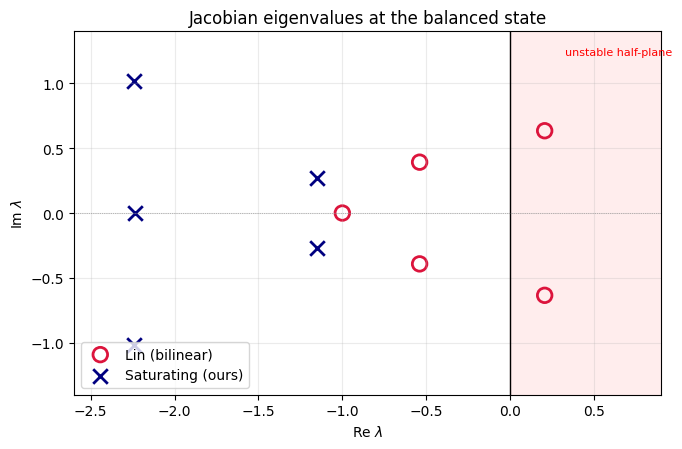
\includegraphics[width=0.68\textwidth]{fig1_eigenvalues.png}
\caption{Jacobian eigenvalues at the balanced state. The shaded region is the
unstable half-plane $\operatorname{Re}\lambda>0$. Two of the five bilinear
eigenvalues lie inside it; all five saturating eigenvalues lie well to the
left.}
\label{fig:eig}
\end{figure}
% ============================================================================
\section{Numerical Results}\label{sec:stability}
% ============================================================================

The eigenvalue computation of Section~\ref{sec:analysis} is a local statement at
one parameter setting. We now test it in three progressively more demanding ways:
by direct perturbation, over two-dimensional regions of parameter space, and over
randomly sampled parameters.

\subsection{Recovery from perturbation}

Stability should mean that the body returns to balance after a disturbance. We
start each model exactly at its balanced state, perturb a single organ, and
integrate. Two perturbation sizes are used: a small one, in which the organ is
raised by five percent, and a severe one, in which it is reduced to thirty
percent of its balanced value, representing a marked deficiency. We measure
\[
\text{deviation}(t) \;=\; \bigl\|\,x(t)-x^\ast\mathbf{1}\,\bigr\|_2 ,
\]
the Euclidean distance of the whole five-organ state from perfect balance.

\begin{table}[!htb]
\centering
\begin{tabular}{llrrl}
\toprule
Model & Perturbation & Initial dev. & Final dev. & Outcome \\
\midrule
Bilinear   & small ($+5\%$)   & $0.0167$ & $0.8776$ & does \textbf{not} recover \\
Bilinear   & severe ($-70\%$) & $0.2333$ & $0.9899$ & does \textbf{not} recover \\
Saturating & small ($+5\%$)   & $0.1335$ & $0.0000$ & recovers \\
Saturating & severe ($-70\%$) & $1.8692$ & $0.0000$ & recovers \\
\bottomrule
\end{tabular}
\caption{Recovery from perturbation of a single organ. In the bilinear model a
five percent disturbance grows by a factor of roughly fifty; in the saturating
model even a severe deficiency is fully corrected by the network.}
\label{tab:pert}
\end{table}

\begin{figure}[!htb]
\centering
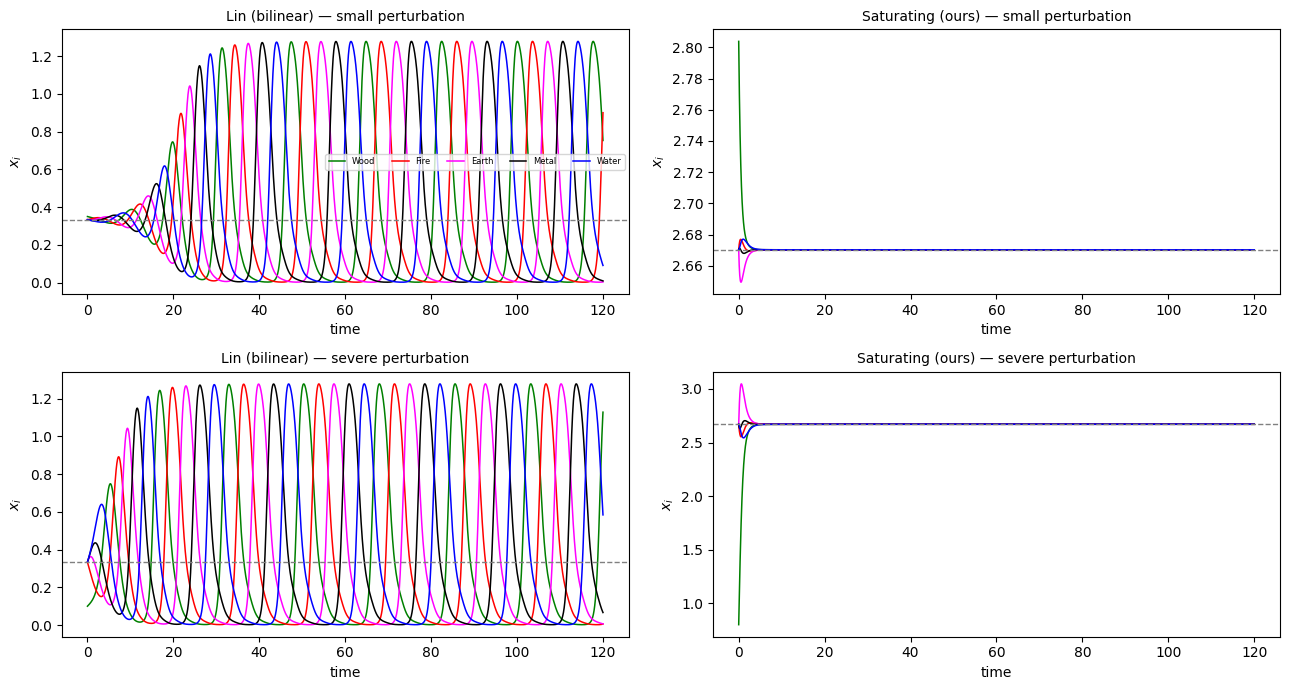
\includegraphics[width=\textwidth]{fig2_perturbation.png}
\caption{Perturbation recovery. The dashed line marks the balanced state. Left
column, bilinear model: the organs leave balance and do not return. Right
column, saturating model: the trajectories return to the line in both cases.}
\label{fig:pert}
\end{figure}

\subsection{No organ is distinguished}

Since the perturbation above is applied to a single organ, it is natural to ask
whether that organ is special. It is not, and this follows from the $\Z_5$
equivariance noted in Section~\ref{sec:analysis}: the wiring is invariant under
$i\mapsto i+1$, so perturbing any organ must produce an identical recovery
curve. We verified this by perturbing each of the five organs in turn. The
spread in final deviation across the five choices is reported in
Table~\ref{tab:z5}; it is at the level of machine precision.

\begin{table}[!htb]
\centering
\begin{tabular}{llc}
\toprule
Model & Perturbation & Spread across organs \\
\midrule
Bilinear   & small  & $1.45\times10^{-14}$ \\
Bilinear   & severe & $1.67\times10^{-15}$ \\
Saturating & small  & $2.52\times10^{-10}$ \\
Saturating & severe & $8.73\times10^{-10}$ \\
\bottomrule
\end{tabular}
\caption{Spread in final deviation across the five choices of perturbed organ.
The agreement confirms $\Z_5$ symmetry and serves as an independent check on the
index maps in the implementation.}
\label{tab:z5}
\end{table}

Beyond closing the objection, this is a useful correctness test: had the index
maps~\eqref{eq:maps} been implemented incorrectly, the symmetry would break and
the five curves would separate.

\subsection{Stability across parameter space}

We next recompute the balanced state, its Jacobian and
$\max_j\operatorname{Re}\lambda_j$ across a grid in two parameters: Sheng
strength against Ke restraint, with the remaining coefficients held at
mid-range values. Because both the equilibrium and the Jacobian are available in
closed form, no differential equation need be solved and the computation is
exact. The contour $\max_j\operatorname{Re}\lambda_j=0$ is the
\emph{stability boundary}.

\begin{figure}[!htb]
\centering
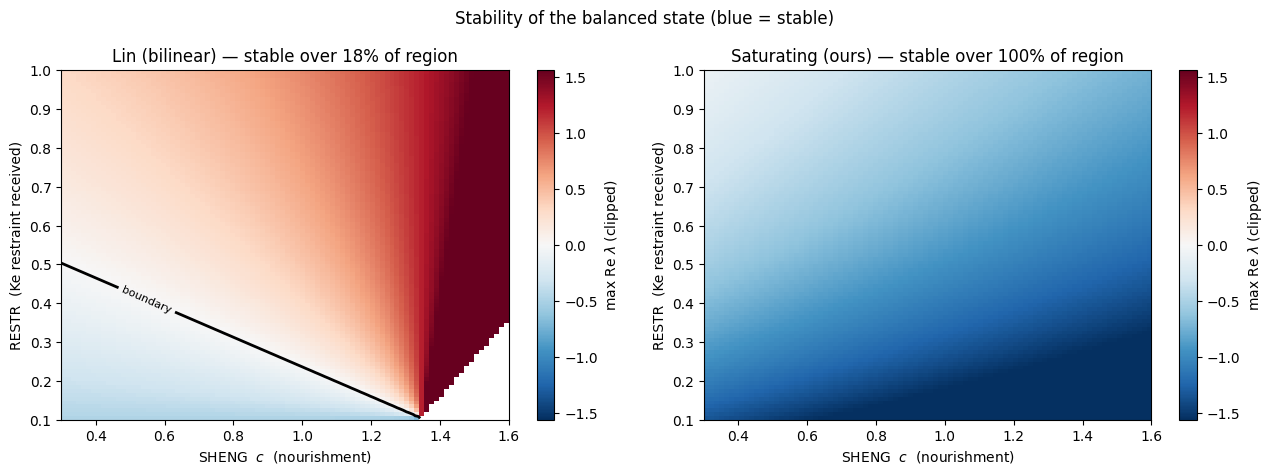
\includegraphics[width=\textwidth]{fig4_stability_maps.png}
\caption{Stability of the balanced state over the plane of Sheng strength
against Ke restraint. Blue indicates stability, red instability, and the black
contour is the stability boundary. The white wedge in the left panel is the
region in which the bilinear model has no positive balanced state. Over this
region the bilinear model is stable in about $18\%$ of cells and the saturating
model in $100\%$.}
\label{fig:stabmap}
\end{figure}

Reading the right-hand panel of Figure~\ref{fig:stabmap}, stability improves as
Sheng strength increases and degrades as Ke restraint increases. This is a
testable prediction of the model, and it agrees with the classical view that
nourishment maintains balance while excessive restraint drives pathology.
Crossing the boundary contour is the model's image of the onset of disease, and
by Remark~\ref{rem:modes} the mode through which the crossing occurs determines
whether the resulting pattern is steady or oscillatory.

% ============================================================================
\section{Randomised Comparison and the Choice of Prior}\label{sec:ordering}
% ============================================================================

The comparisons so far fix all but two parameters. To remove any suspicion that
the conclusion depends on a fortunate choice, we sample parameters at random and
count how often each model has a stable balanced state.

\subsection{Concept mapping and fairness}

The two models name the same physiological quantities differently, so we sample
\emph{concepts} and hand each model the coefficients it requires
(Table~\ref{tab:concepts}). Both models therefore receive the same physiological
draw.

\begin{table}[!htb]
\centering
\begin{tabular}{llcc}
\toprule
Concept & Meaning & Bilinear & Saturating \\
\midrule
\texttt{SELF}  & self-production                       & $a$ & $a$ \\
\texttt{SAT}   & self-limitation                       & $b$ & $k$ \\
\texttt{SHENG} & nourishment received from the mother  & $c$ & $c$ \\
\texttt{RESTR} & Ke restraint received from controller & $d$ & $h$ \\
\texttt{TGT}   & cost associated with the Ke target    & $h$ & $g$ \\
\texttt{CHILD} & cost of nourishing the child          & $g$ & --- \\
\bottomrule
\end{tabular}
\caption{Correspondence between the coefficients of the two models.}
\label{tab:concepts}
\end{table}

Two further precautions are taken. First, the balanced state of the bilinear
model exists only when $M=b+d+g+h-c>0$; draws violating this are discarded, so
that the model is scored only where it is well posed. Second, we report the
stability fraction both as a proportion of \emph{valid} draws and as a
proportion of \emph{all} draws, so that nothing is concealed by the filtering.
The stability fraction is defined as
\[
\text{stability fraction}=
\frac{\#\{\text{draws whose balanced state satisfies } \max_j\operatorname{Re}\lambda_j<0\}}
     {\#\{\text{draws possessing a positive balanced state}\}} .
\]

\subsection{A physiologically justified ordering}

Drawing every coefficient from a common range is not physiologically neutral: it
treats self-production and pathological over-acting as equally likely to
dominate. We therefore also sample under the ordering
\begin{equation}\label{eq:order}
\texttt{SELF} \;>\; \texttt{SHENG} \;>\; \texttt{RESTR} \;>\; \texttt{TGT},
\end{equation}
justified as follows.

\begin{enumerate}
\item \textbf{\texttt{SELF} is largest.} Each organ possesses its own 正气, which
is the primary source of its function; the inter-organ relations \emph{modulate}
that baseline rather than supply it. This is also a viability requirement: were
the losses to exceed self-production, the organ could not maintain activity.

\item \textbf{\texttt{SHENG} exceeds \texttt{RESTR}.} Sheng is the nourishing
relation that sustains activity, whereas Ke is a brake: under normal conditions
the restraint is required to keep the target from growing without bound
(relation~6 of Section~\ref{sec:relations}). A brake that exceeds the engine is
not a regulator but a shutdown, so for a viable network nourishment must dominate
restraint.

\item \textbf{\texttt{RESTR} exceeds \texttt{TGT}.} Ordinary Ke restraint is
physiological and always present, whereas over-acting (相乘) is a
\emph{pathological deviation} arising when the controller is in excess or the
target deficient. In a broadly healthy body the normal relation should outweigh
the pathological one.

\item \textbf{The classical grading of the abnormal relations.} Where the Wu term
is included, the classics rank 相乘 (贼邪, which \emph{greatly} weakens) above
相侮 (微邪, which only \emph{mildly} weakens), so the rebellion coefficient should
be the smallest of all. The model analysed here has no Wu term, so this
constraint is recorded for use in the extended model rather than applied now.
\end{enumerate}

It is important that this ordering is justified on physiological grounds
\emph{alone}, before any stability computation. Otherwise the argument would be
circular.

We implement~\eqref{eq:order} in two ways: by rejection, keeping only draws that
satisfy the chain while all marginal ranges remain identical; and by assigning
each concept its own range (\texttt{SELF} $\in[1.0,2.0]$, \texttt{SHENG}
$\in[0.5,1.5]$, \texttt{SAT} $\in[0.3,1.0]$, \texttt{RESTR} $\in[0.2,0.8]$,
\texttt{TGT} and \texttt{CHILD} $\in[0.1,0.5]$).

\subsection{Results}

\begin{table}[!htb]
\centering
\begin{tabular}{lcc}
\toprule
Sampling prior & Bilinear (95\% CI) & Saturating (95\% CI) \\
\midrule
uniform (naive)  & $22.8\%$ $[20.6,\,25.3]$ & $94.1\%$ $[92.5,\,95.4]$ \\
full ordering    & $47.1\%$ $[44.3,\,50.0]$ & $91.9\%$ $[90.2,\,93.3]$ \\
tiered ranges    & $23.3\%$ $[21.0,\,25.9]$ & $99.0\%$ $[98.3,\,99.4]$ \\
\bottomrule
\end{tabular}
\caption{Proportion of random parameter draws for which the balanced state is
asymptotically stable, with Wilson $95\%$ confidence intervals. The intervals do
not overlap under any prior.}
\label{tab:mc}
\end{table}

\begin{figure}[!htb]
\centering
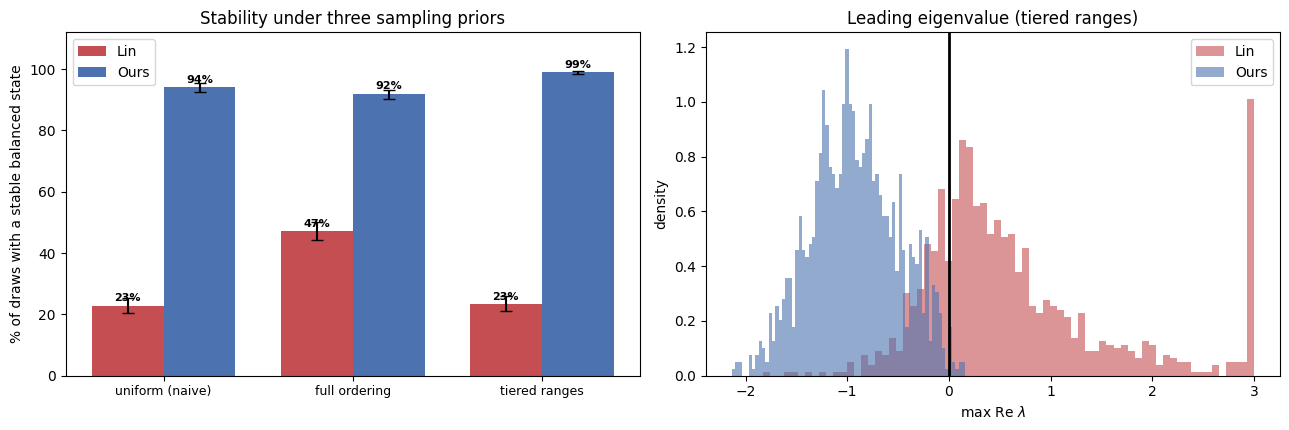
\includegraphics[width=\textwidth]{fig6_sampling_comparison.png}
\caption{Left: stability fraction under three sampling priors, with Wilson
confidence intervals. Right: distribution of $\max_j\operatorname{Re}\lambda_j$
under the tiered ranges; the saturating distribution lies almost entirely to the
left of zero.}
\label{fig:mc}
\end{figure}

\paragraph{The ordering favours the competing model.}
The most important observation in Table~\ref{tab:mc} is that imposing the
physiological ordering roughly \emph{doubles} the bilinear model's stability
fraction, from $22.8\%$ to $47.1\%$, while slightly \emph{reducing} that of the
saturating model, from $94.1\%$ to $91.9\%$. The ordering is therefore not a
device that flatters our model; it corrects an unfairness in the naive prior.
The comparison under the ordered prior is consequently the conservative one, and
we recommend that the figures $47.1\%$ against $91.9\%$ be taken as the headline
result. We regard the fact that a prior derived purely from physiological
reasoning happens to move the bilinear model towards sustaining balance as weak
independent evidence that the ordering identifies biologically meaningful
regions of parameter space.

\subsection{Behaviour when balance fails}

Stability tells us whether the balanced state holds; it does not say what
happens instead when it does not. We therefore classify the long-run behaviour of
each random draw as a fixed point, a periodic orbit, chaos, or blow-up, using the
regularity of successive peaks of one coordinate after discarding a transient.

\begin{remark}[Dependence on initial conditions]\label{rem:ic}
A nonlinear system may possess several attractors simultaneously, so a
classification made from a single starting point describes that trajectory
rather than the model. We therefore classify from three initial conditions and
count over all pairs of parameter set and starting point. This matters
substantially: across the draws examined, all three starting points agreed for
the saturating model in $100\%$ of cases but for the bilinear model in only
$18\%$. The start-independence of the saturating model is itself a result, and
the corresponding figures for the bilinear model must be read as
start-sensitive.
\end{remark}

\begin{table}[!htb]
\centering
\begin{tabular}{lcc}
\toprule
Long-run behaviour & Bilinear & Saturating \\
\midrule
fixed point & $45\%$ & $100\%$ \\
periodic    & $52\%$ & $0\%$ \\
chaotic     & $2\%$  & $0\%$ \\
blow-up     & $2\%$  & $0\%$ \\
\bottomrule
\end{tabular}
\caption{Long-run behaviour over pairs of randomly drawn parameter set and
initial condition, under the tiered ranges.}
\label{tab:regime}
\end{table}

\begin{figure}[!htb]
\centering
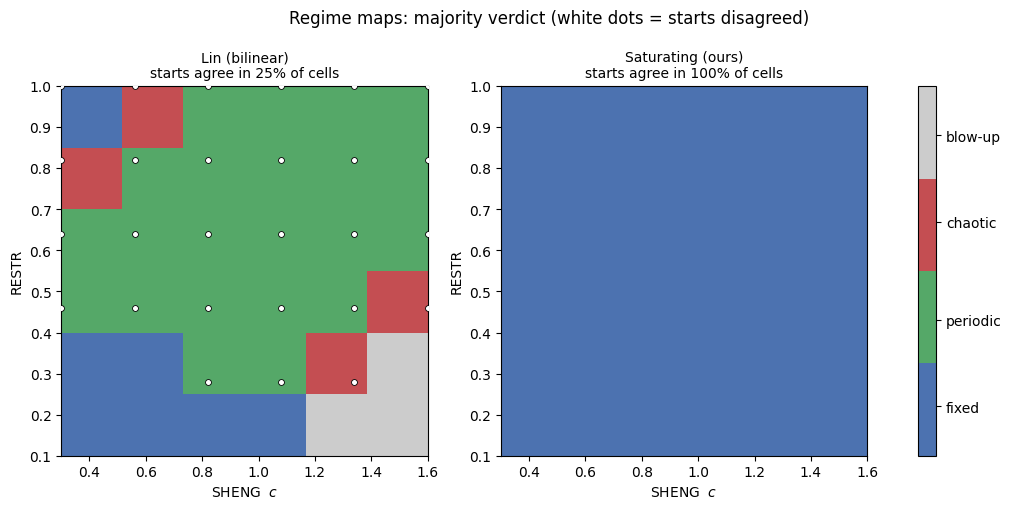
\includegraphics[width=\textwidth]{fig5_regime_maps_multiIC.png}
\caption{Regime maps showing the majority verdict over three initial conditions.
White dots mark cells in which the initial conditions disagreed. The starting
point determines the verdict in only $25\%$ of cells for the bilinear model,
against $100\%$ for the saturating model.}
\label{fig:regime}
\end{figure}

\subsection{Is the bilinear model handicapped by its extra term?}

The bilinear model carries six coefficients and the saturating model five: the
former includes \texttt{CHILD}, the cost of nourishing one's child, which the
latter omits. It is reasonable to ask whether we are penalising the bilinear
model for carrying a loss term absent from ours. We tested this by setting
\texttt{CHILD} to zero and re-scoring.

\begin{table}[!htb]
\centering
\begin{tabular}{lc}
\toprule
Model & Stability fraction \\
\midrule
Bilinear, all six terms       & $22.1\%$ \\
Bilinear, \texttt{CHILD} removed & $12.0\%$ \\
Saturating, five terms        & $94.8\%$ \\
\bottomrule
\end{tabular}
\caption{Ablation of the extra bilinear term. Removing it makes the bilinear
model \emph{worse}, so the term is an advantage rather than a handicap.}
\label{tab:ablation}
\end{table}

Removing the term lowers the bilinear stability fraction from $22.1\%$ to
$12.0\%$. The sixth term therefore \emph{helps} the bilinear model, so carrying
it is an advantage and not a handicap; the comparison is generous to the
competing model rather than unfair to it.

% ============================================================================
\section{Limitations}\label{sec:limits}
% ============================================================================

We state the weaknesses of each test explicitly.

\paragraph{Local versus global stability.}
The eigenvalue criterion is local: it establishes that small disturbances decay
but says nothing about the size of the basin of attraction. The perturbation
experiments of Section~\ref{sec:stability} partially address this, since the
severe perturbation is large, but they examine only two disturbance magnitudes.
As a partial validation we compared the eigenvalue verdict against direct
simulation over $120$ random draws per model: the two agreed in $98.3\%$ of
bilinear cases and $100\%$ of saturating cases, with every disagreement occurring
at $|\max_j\operatorname{Re}\lambda_j|<0.011$, that is, in marginal cases whose
convergence is slower than the integration window.

\paragraph{Choice of prior.}
There is no canonical prior over these coefficients. Uniform sampling is a
choice, and the tier boundaries are a judgement. We mitigate this by reporting
three priors and by checking that the conclusion survives rescaling the tier
widths, but the issue cannot be eliminated. This is why the ordered prior, which
is the least favourable to our conclusion, is quoted as the headline.

\paragraph{Unequal parameter counts.}
The two models do not have identical parameter spaces, and the concept mapping of
Table~\ref{tab:concepts} is a modelling judgement. The ablation of
Table~\ref{tab:ablation} shows that the asymmetry favours the bilinear model.

\paragraph{Existence filtering.}
The saturating model has no positive balanced state when $a+c\le g$, which
occurred in roughly $14\%$ of naive draws. Such draws are excluded from the
conditional fraction and included in the unconditional one; both are reported.

\paragraph{Regime classification.}
The classifier uses thresholds chosen by us, and the label ``chaotic'' should be
read as ``bounded and irregular'': Lyapunov exponents were not computed for every
draw. As noted in Remark~\ref{rem:ic}, the classification is also
start-sensitive for the bilinear model.

\paragraph{The modelling assumption itself.}
Identifying health with a stable \emph{symmetric} equilibrium is an assumption.
A real body is not perfectly symmetric, and one might argue that health is better
represented by a bounded oscillation than by a fixed point. Our results should be
read as establishing that the saturating model \emph{can} represent a stable
balanced state while the bilinear model essentially cannot, not as establishing
that a fixed point is the only admissible notion of health.

% ============================================================================
\section{Network Motifs}\label{sec:motifs}
% ============================================================================

\RED{[To be written. This section will develop the interpretation of the
classical treatment principles as statements about small subnetworks: the
one-node self-regulation motif, the two-node Sheng (mother--child) and Ke
(controller--target) motifs, and the three-node motif underlying the principle of
strengthening the organ that a diseased organ will next attack. The key
observations to develop are that every classical principle---虚则补其母,
实则泻其子, 母能令子虚, 子能令母实, and the abnormal relations 相乘 and
相侮---names only two or three organs, so that TCM is implicitly a motif theory
of physiology; and that such local reasoning is mathematically justified exactly
when the coupling to the remainder of the network is weak or slow, which is a
statement about separation of time scales and is testable in the present model.
The circulant structure of Section~\ref{sec:analysis} and the mode
decomposition of Remark~\ref{rem:modes} provide the natural bridge between the
local motifs and the global five-node dynamics.]}

% ============================================================================
\section{Discussion}\label{sec:discussion}
% ============================================================================

The central finding of this paper is that a single modelling choice---whether
inter-organ interactions saturate---determines whether the five-element system
can represent sustained health.

In the bilinear formulation, nourishment delivered to an organ is proportional to
the product of mother and child. This has two consequences. Physiologically, it
inverts the classical relation: a depleted child receives \emph{less}
nourishment rather than more, whereas the classics assert that a weak child draws
harder on its mother. Dynamically, the coupling is unbounded, so it can outrun
the quadratic self-limitation; the balanced state is generically unstable, and
outside the region $M>0$ solutions diverge in finite time.

Replacing the coupling by a saturating one repairs both. The demand factor
$1/(1+x_i)$ makes nourishment largest exactly when the child is most depleted,
which is what relation~1 requires, and it bounds the interaction, so that the
quadratic term always eventually dominates. The result is the invariant box of
Proposition~\ref{prop:box}, positivity and boundedness for all parameters, and a
balanced state that is stable over most of parameter space.

We emphasise that the corrections of Section~\ref{sec:corrections} do not
undermine the earlier work so much as sharpen it. Lin and Han's central
qualitative claims---that the system exhibits fixed points, cycles and irregular
motion, and that the symmetric equilibrium of their model is unstable---survive.
What changes is the classification of particular cases, and in each instance the
correction makes their model better behaved than reported, not worse. The
conclusion that the bilinear balanced state is unstable is unaffected, since it
follows directly from the eigenvalues $0.206\pm0.634i$, which we reproduce
exactly.

The circulant structure deserves emphasis beyond its computational convenience.
Because the Fourier modes split into a uniform mode and four symmetry-breaking
modes, the model distinguishes automatically between a body that is uniformly
depleted or uniformly over-active and one that has developed a specific pattern
of excess and deficiency across organs. The latter is what TCM diagnosis
actually identifies. Which mode loses stability first therefore predicts
\emph{which kind} of disorder the model develops, and the $\Z_5$ symmetry
constrains the possible patterns.

% ============================================================================
\section{Future Work}\label{sec:future}
% ============================================================================

\begin{enumerate}
\item \textbf{Disease propagation.} Perturbing a single organ and tracking the
propagation of the disturbance along the Ke cycle would allow a direct test of
the classical instruction to strengthen the organ that the diseased organ will
attack next, before treating the diseased organ itself.

\item \textbf{The named pathologies.} The model should be shown to reproduce
母病及子, 子盗母气, 相乘 and 相侮 as time-dependent behaviour. Capturing the
mother-consumption relations~4 and~5 requires adding to the mother's equation a
term matching the child's draw, of the form $-g_{\sigma}x_{\sigma(i)}/(1+x_i)$,
which makes the Sheng coupling bidirectional.

\item \textbf{Rebellion and adaptive set points.} Reinstating the Wu term, and
allowing the homeostatic target itself to depend on the organ's neighbours
through $\theta_i=\theta_i^0+\alpha_i x_{\sigma(i)}-\beta_i x_{\rho(i)}$, gives
two further model variants to which the present pipeline applies unchanged. The
classical grading 相乘 $>$ 相侮 then becomes an active constraint on the
coefficients.

\item \textbf{Bifurcation analysis.} Continuation of the stability boundary of
Figure~\ref{fig:stabmap} in two parameters would classify the crossings as steady
symmetry-breaking or Hopf, and $\Z_5$-equivariant bifurcation theory predicts
which symmetry-broken patterns arise. The staggered wave observed in the bilinear
periodic solution is a rotating wave in this language.

\item \textbf{Treatment as control.} The intervention terms $e_i$ set to zero
in~\cite{Lin2020} can be reinstated as control inputs, turning the model into a
tool for treatment design: one asks for the minimal intervention that returns a
diseased trajectory to the basin of the balanced state. This corresponds directly
to the classical principles of tonifying the mother and draining the child.
\end{enumerate}

% ============================================================================
\section*{Reproducibility}
% ============================================================================

All numerical results in this paper were produced by scripts that regenerate
every figure and table from scratch. The Jacobians were validated against finite
differences, the equilibrium formulae by substitution, and the eigenvalue-based
stability verdict against direct simulation. Random draws are seeded; repeating
the study with five different seeds changed the bilinear stability fraction only
within $22.8\%$--$24.0\%$ and the saturating fraction within $94.6\%$--$96.1\%$.

\printbibliography

\end{document}
